

\vspace{-.5em}
\section{Query Processing on Dirty Data}\label{sec:error}
Like other \saqp systems, our main focus is on aggregate numerical queries (\avgfunc, \sumfunc, \countfunc, \var, \geomeanfunc, \productfunc) of the form:
\begin{alltt}
SELECT \textsf{f}(attrs) FROM table \\WHERE predicate \\GROUP BY attrs
\end{alltt}
%We defer the implementation of more complex SQL operators such as joins and nested queries for future work.
When running the aggregate queries on large and dirty datasets, there may be two separate sources of errors that affect result quality. (1) Sampling error: since data is large, we may execute queries on a sample of the data to reduce query times. (2) Data error: since real-world data is dirty, queries on the dirty data also lead to inaccurate query results. 

In this section, we first precisely characterize sampling and data errors, and then present our \saqpplus framework to deal with these two types of errors.
Throughout the section, we will refer to the following example query on a dataset of academic publications:
\begin{alltt}
SELECT \textsf{AVG}(citation_count) FROM papers \\GROUP BY pub_year
\end{alltt}
which finds the average number of citations of the publications published every year.

\iffalse
Throughout the section, we will refer to the following example query on a dataset of academic publications:
\begin{alltt}
SELECT \textsf{AVG}(citation_count) FROM papers \\WHERE pub_year>2000
\end{alltt}
which finds the average number of citations received by the publications published after the year 2000.
\fi

\subsection{Sampling Error}\label{subsec:saqp}
There are many different ways to sample data; a data sample could be either created online during the query time~\cite{DBLP:conf/sigmod/HellersteinHW97,DBLP:journals/pvldb/PansareBJC11,DBLP:conf/sigmod/CondieCAHGTES10,DBLP:journals/pvldb/WuJOT09} or built offline from past query workloads~\cite{DBLP:conf/eurosys/AgarwalMPMMS13,DBLP:conf/sigmod/AcharyaGPR99,DBLP:journals/tods/ChaudhuriDN07,DBLP:conf/sigmod/BabcockCD03}.  
Consider our example citation query.
A uniform random-sampling scheme randomly selects a set of papers from \texttt{papers} such that every paper has an equal probability of selection.
%This sampling scheme is not a good choice for a \groupby query since the number of papers published in each year may differ a lot.
%At worst, it will lead to some years with no paper in the sample data.
To answer queries with a highly selective predicate or a \groupby clause, prior works employ stratified-sampling ~\cite{DBLP:conf/sigmod/HellersteinHW97,DBLP:conf/sigmod/AcharyaGP00,DBLP:conf/eurosys/AgarwalMPMMS13}, which performs a uniform random sampling scheme in each group, to guarantee that every group has a large enough sample size to estimate a good result. 
The approaches presented in this paper can support both uniformly random samples and stratified samples.
However, for simplicity, we present our analysis with uniform samples.

Answering queries on a sample has an inherent uncertainty since a different sample may yield a different result.
Quantifying this uncertainty has been extensively studied in statistics~\cite{lohr2010sampling}.
Due to this uncertainty, we return confidence intervals in addition to results.
For example, given a confidence probability (e.g., 95\%), we can apply results from sampling statistics to estimate the average number of citations along with a confidence interval (e.g. $\pm10$), which means that the estimated average number is within $\pm10$ of the actual value with 95\% probability.
The confidence interval quantifies the uncertainty introduced by sampling the data.




%For ease of presentation, we introduce some notations and terminology.

%The basic idea of \saqp is to sample the data, then run the aggregate queries on the sample to obtain approximate results, and finally provide a confidence interval bounding the approximate result.
%Since the query is only run on the sample data instead of the entire data, the query time can be significantly reduced.
%There are two key components of \saqp systems: sample creation and result estimation.
 
%\vspace{.5em}

%{\noindent \bf Sample Creation:} According to different application requirements, a data sample could be either created online during the query time~\cite{DBLP:conf/sigmod/HellersteinHW97,DBLP:journals/pvldb/PansareBJC11,DBLP:conf/sigmod/CondieCAHGTES10,DBLP:journals/pvldb/WuJOT09} or built offline based on query workloads~\cite{DBLP:conf/eurosys/AgarwalMPMMS13,DBLP:conf/sigmod/AcharyaGPR99,DBLP:journals/tods/ChaudhuriDN07,DBLP:conf/sigmod/BabcockCD03}. In comparison, the online sampling has more flexibility to derive an estimate result while the offline sampling can save the sampling time from the query time. 
%
%Consider the query in the beginning of this section. A simple-random-sampling scheme is to randomly select a set of papers from \texttt{papers} such that every paper has the equal probability of the selection. This sampling scheme is not a good choice for a \groupby query since the number of papers published in each year may differ a lot. At worst, it will lead to some years with no paper in the sample data. To avoid this problem, the prior works typically adopt a stratified-sampling scheme~\cite{DBLP:conf/sigmod/HellersteinHW97,DBLP:conf/sigmod/AcharyaGP00,DBLP:conf/eurosys/AgarwalMPMMS13}, which performs a simple-random-sampling scheme in each group, to guarantee that every group has a large enough sample size to estimate a good result. 
%In our paper, we choose the online sampling since we will use the crowd to clean the sample, and the query time is mainly dominated by the crowd-cleaning time. Next, we introduce how to use the online sampling to create a sample for a \groupby query. 


\subsection{Data Error}\label{subsec:dataclean}
In this work, we focus on three types of data errors: \verror, \cerror, and \derror.
We use our example query to illustrate how these errors can affect results.
%Let $\gfunc_{a}(\cdot)$ denote an aggregation function, where $a$ represents an aggregation attribute. (We will often omit $a$ in the function if it is clear from the context.) For example, the aggregation function, $\avgfunc_{\textrm{citation}}(\Pset)$, computes the average number of citations of the papers in $\Pset$.  

%sample data $\Sseti{i}$ randomly drawn from $\Pseti{i}$. For each tuple $t\in \Sseti{i}$, we model its cleaning results as follows:

\vspace{.5em}

\begin{figure}[tup] % \vspace{-1em}
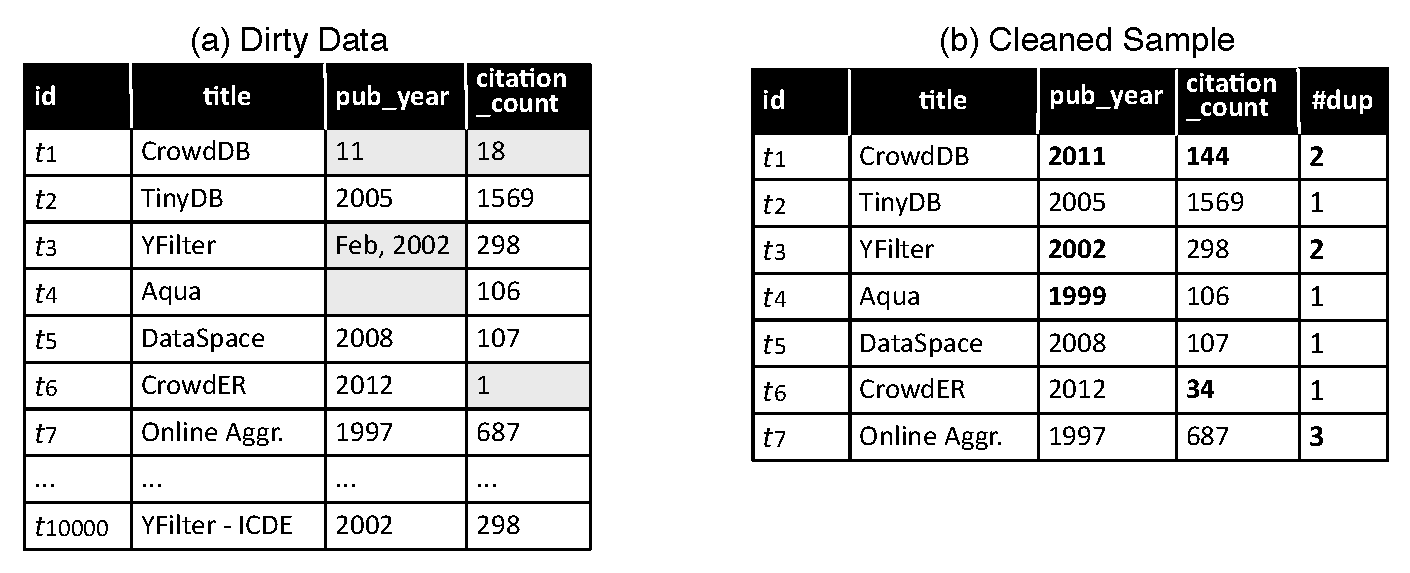
\includegraphics[scale=0.35]{figs/new-example.pdf}\vspace{-1em}
\caption{An example of dirty data and cleaned sample (Shaded cells denote dirty values, and their cleaned values are in bold font).}\vspace{-1.5em}
\label{fig:example}
\end{figure}

{\noindent \bf \Verror:} When an error occurs in the aggregation attributes of the query (i.e. \texttt{citation\_count}), it will lead to an incorrect aggregate result. For example, consider the dirty data in Figure~\ref{fig:example}(a). The first paper $t_1$ involves \verror since its citation count should be 144 instead of 18. %We use $\Correct{t}$ to denote the tuple's correct aggregation-attribute value.  


%Many data-cleaning techniques, such as outlier detection~\cite{hellerstein2008quantitative,DBLP:conf/pervasive/JefferyAFHW06} or rule-based approaches~\cite{fan2012foundations,DBLP:conf/sigmod/DallachiesaEEEIOT13}, have been proposed. We use $\Correct{t}$ to denote the correct aggregation-attribute value of the tuple $t$.  

\vspace{.5em}

{\noindent \bf \Cerror:} When an error occurs in the predicate or group-by attribute of the query (i.e. \texttt{pub\_year}), there may be some tuples that are \emph{falsely} added into or excluded from a group, leading to an incorrect result. In Figure~\ref{fig:example}(a), the first paper $t_1$ also has \cerror since it was published in the year 2011 rather than 11. %Note that this type of error can also be extended to errors in \groupby attributes (refer to Section \ref{sec:query-processing} for details).

%We use $\Predicate{t}$=True ($\Predicate{t}$=False) to denote the cleaned tuple satisfy (dissatisfy) the predicate.


\vspace{.5em}

{\noindent \bf \Derror:} If data contains duplicate tuples (e.g., different representations of the same paper), the aggregate result will also be affected. This type of error commonly happens when the data is integrated from multiple sources. For instance, in Figure~\ref{fig:example}(a), the third paper $t_3$ has \derror as it refers to the same paper as $t_{10000}$.  %We use $\Dedup{t}{\Pset}$ to denote the number of duplicate tuples of $t$ in the dirty data (including $t$ itself).

\vspace{.5em}




%The errors rate (fraction of tuples affected) can vary as well. In this work, we classify \emph{error regimes} by the error rate ranging from 0\% (all of the tuples clean) to 100\% (all of the tuples dirty) for each type of error. Accordingly, we explore how these different regimes affect aggregate query results and our choice of estimation method.

%\Verror and \cerror are both caused by the incorrect attribute values of the dirty data. Many data-cleaning techniques, such as outlier detection~\cite{hellerstein2008quantitative,DBLP:conf/pervasive/JefferyAFHW06} or rule-based approaches~\cite{fan2012foundations,DBLP:conf/sigmod/DallachiesaEEEIOT13}, have been proposed to solve this problem. For example, Fan et al.~\cite{DBLP:journals/pvldb/FanLMTY10} proposed editing rules, master data and user confirmation to correct attribute values, and they proved that their approaches can always obtain reliable cleaning results.

%There are also many studies in dealing with the duplication error (see~\cite{DBLP:journals/tkde/ElmagarmidIV07} for a survey). Particularly, recent work explores the use of crowdsourcing to solve this problem. For example, Wang et al.~\cite{DBLP:journals/pvldb/WangKFF12} proposed a hybrid human-machine framework, which first adopts machine-based techniques to filter obviously non-duplicate tuples for each tuple, and then utilizes the crowd to check the remaining ones. 

While data cleaning can fix the data errors, cleaning the entire data is usually time consuming, often requiring user confirmation or crowdsourcing. For this reason, we have developed the \saqpplus framework.















%Therefore, if it is possible to only clean a sample of the data (i.e., correct the attribute values in the sample, and find the number of duplicate tuples for each tuple in the sample), all of the above .


%Note that the main focus of this work is not on a specific data-cleaning. our work is orthogonal to data-cleaning technique to use. In fact, 




%Note that to compute $\Dedup{t}{\Pset}$, we do not need to compare $t$ with every tuple in the data. Most existing deduplication approaches first employ machine-based techniques~\cite{journals/tkde/Christen11} to identify a candidate set of tuples for $t$, and then only compare $t$ with the candidate tuples. Typically, the number of candidate tuples is much smaller than the whole data size, and scales well with large data sets.




%It is worth mentioning that the above cleaning results cannot capture the missing tuples of the population, i.e. \emph{false-negative error}. For example, there might be some papers that were actually published by ``UC Berkeley" after 2000, but due to the errors in their ``year" or ``university" attributes (e.g., ``year" values are missing or ``UC Berkeley" is represented as ``UCB"), they were not added into the population. As it is hard to know which tuples are missing in the population, in our paper, we assume there is no false-negative error in the population. In practice, to avoid false-negative error, users can create a population by adding all \emph{possible} tuples in it, and transform false-negative error into false-positive error. For example, they can assume all the missing ``year" values satisfy the predicate, and add the corresponding papers (e.g., $t_3$ and $t_4$ in Figure~\ref{fig:example}) into the population. Although some papers may be falsely added into the population, they can use the data-cleaning techniques for the false-positive error to remove such papers (e.g., $t_4$). 

%We assume users should handle such error by themselves. For example, when issuing the query, users can add ``\texttt{or year is NULL}" into the predicate to include the papers whose ``year" values are missing, and then utilize the crowd cleaning (i.e., $\Remove{t}{\Pseti{i}}$) to remove the falsely included papers. They can also identify different representations of ``UC Berkeley" in the ``university" attribute, and add the corresponding tuples into the population w.r.t ``UC Berkeley". Note that the distinct number of \groupby keys is typically much smaller than the number of tuples in the data.

\iffalse
When running the above query on a dirty table, we may get a different result than running on the real clean one. In this section, we analyze what types of data errors will affect the query result, and classify them into three classes: 

\mbox{}

{\noindent \bf Aggregation Error:} When there are incorrect values in aggregate attributes, we call such error as aggregation error. For example, consider the query in Example 1. The citation of Paper 2 in Table 1 is an aggregation error since citation is an aggregate attribute, and the citation number is incorrect and should be 234.


\vspace{.5em}

{\noindent \bf Predicate Error:} Predicate error is caused by the incorrect values in predicate attributes. There are two types of predicate errors: false positive error and false negative error. The former one refers to the tuples that violate the predicate, but falsely identify as satisfying the predicate. The latter one refers to the tuples that satisfy the predicate, but falsely identify as violating the predicate.  



\vspace{.5em}


{\noindent \bf Duplication Error:} 

\mbox{}


Three types of data errors:
\begin{itemize}
  \item {\bf Aggregation Error:} Incorrect values in aggregation attributes
  \item {\bf Predicate Error:} The tuples that satisfy the predicate in the query may not be what users want.
  \item {\bf Duplication Error:} Duplicate tuples in the data
\end{itemize}
\fi

\iffalse
\subsection{Problem Formulation}\label{subsec:problem}
Now we formulate our problem in this section. Given a set of populations that may contain data errors, by cleaning more data, we can estimate a better aggregation result. Since it is expensive to clean the entire data, we investigate how to achieve satisfied result quality by only cleaning a sample of data. Specifically, we study the following two problems:

\vspace{.5em}

{\noindent \bf Quality-constrained problem:} We allow users to specify a constraint of result quality, and aim to clean the minimum number of tuples to satisfy the constraint. The result-quality constraint is defined as an error bound along with a confidence probability. Note that our goal is to estimate the aggregation result for each cleaned population rather than the original (dirty) population. Let $\PCseti{i}$ ($i\in[1,M]$) denote the corresponding cleaned population to $\Pseti{i}$. When we say the estimated result satisfies the quality constraint, it means that the error bar of the estimated result of each $\PCseti{i}$ ($i\in[1,M]$) is smaller than the given error bound with the confidence probability. We formulate this problem as follows:

\begin{definition}
Given a set of populations, an aggregation function, an aggregation attribute, and a result-quality constraint, the goal of quality-constrained problem is to clean the minimum number of tuples in order to make the estimated result of each cleaned population satisfy the quality constraint.
\end{definition}


\vspace{.5em}

{\noindent \bf Cost-constrained problem:} We also allow users to specify a constraint of cleaning cost, and aim to achieve the best result quality within the cleaning cost. The cleaning-cost constraint is defined as the total number of tuples that can be cleaned. For each population, if we can clean more tuples, its result can be estimated more accurately. Therefore, in order to better balance the result quality of different populations, we define the overall quality of all populations as the worst one (with the largest error bar) among them, and study how to determine the number of tuples cleaned for each population to minimize the largest error bar. We formulate this problem as follows:



\begin{definition}
Given a set of populations, an aggregation function, an aggregation attribute, and a cleaning-cost constraint, the goal of cost-constrained problem is to estimate a result for each cleaned population in order to achieve the best overall quality within the cleaning-cost constraint.
\end{definition}


\begin{example}\label{exa:problem-formulation}
Consider two populations, $\Pseti{1}$ w.r.t ``UC Berkeley" and  $\Pseti{2}$ w.r.t ``Stanford". Suppose we want to compute the average citation of the papers in each population. Thus, the aggregation function is \attr{citation} and the aggregation function is \afunc{AVG}. 

Given a result-quality constraint (e.g., error bound: 1\% and confidence probability: 95\%), we then clean the papers in $\Pseti{1}$ and $\Pseti{2}$ to achieve such quality. For instance, after cleaning 1000 papers in $\Pseti{1}$ and 1500 papers in $\Pseti{2}$, assume the estimated average citation of the cleaned $\Pseti{1}$ (i.e., $\PCseti{1}$) is 200 with $\pm0.8\%$ error bar, and the estimated average citation of $\PCseti{2}$ is 180 with $\pm 3\%$ error bar. Since ``UC Berkeley" has already satisfied the quality constraint (i.e. 0.8\% < 1\%), we can stop to clean its papers. But for ``Stanford", we still need to clean its papers until its error becomes smaller than~1\%. 

Given a cost-quality constraint (e.g., 2500 tuples), we then clean at most 2500 tuples in order to achieve the best overall quality. For the above example, if we clean 1000 papers in $\Pseti{1}$ and 1500 papers in $\Pseti{2}$, based on the definition of the overall quality, it will be equal to 3\% that is the error of ``Stanford". Since the error of ``UC Berkeley" is only 0.8\%, it would be better to reduce the number of cleaned tuples for ``UC Berkeley", and save such tuples to clean more tuples for ``Stanford". 
\end{example}

\fi
\iffalse




When the data is clean, it is easy to estimate the aggregation result based on the sample data using existing approaches. However, when the data becomes dirty, the problem becomes challenging since we need to estimate the aggregation result of the entire clean data based on a sample of cleaned data.

Prior \saqp systems assume data is clean, and utilize existing statistical tools to estimate the result based on the sample data. While the data becomes dirty, 

After the crowd has cleaned the sample data, the key problem is how to estimate the aggregation result of the whole clean data based on the cleaned sample data. Next we formulate this problem.

Let $\PCset$ denote the cleaned population set corresponding to $\Pset$. Let $\gfunc(\cdot)$ denote an aggregation function such as $mean(\cdot)$, $sum(\cdot)$ and $count(\cdot)$. Our goal is to estimate the aggregation result of the whole clean data, i.e., $\gfunc(\PCset[a])$, where $\PCset[a] = \{t[a]~|~t\in\PCset\}$ represents the set of aggregation-attribute values in $\PCset$.

\begin{definition}
Given a sample set $\Sset$ randomly drawn from $\Pset$, the crowd-cleaning results $\Correct{t[a]}$, $\Remove{t}{\Pset}$
$\Dedup{t}{\Pset}$ for each tuple $t\in\Sset$, and a confidence probability, we aim to compute (1) an unbiased estimation result of the entire clean data, and (2) an error bound with the specified confidence probability.
\end{definition}







an error-bound constraint with a confidence value

\begin{definition}
Given $M$ population sets, and a cleaning-cost constraint, \projx aims to decide the number of cleaned tuples for each population set such that the 
\end{definition}


For ease of presentation, we assume the query only has aggregate and predicate attributes in the later text. We discuss how \projx processes the query with grouping attributes in Section~\ref{sec:extension}. 


Users are allowed to add time, cost and quality constraints to the query. BlinkDB~\cite{??} has the query language to support time and quality constraints. We extend its language with the cost constraint. For example, a user may want to get the most accurate result within $t$ minutes by at most cleaning $c$ tuples, then she can run the following query:
\begin{alltt}
SELECT Aggregate(\(A\sb{a}\)) FROM \(T\)
WHERE Predicate(\(A\sb{p}\))
WITHIN COST \(c\) TUPLES, TIME \(t\) MINUTES
\end{alltt}
Or given a quality constraint, a user may want to clean the minimum number of tuples to satisfy the quality constraint, then she can run the following query:
\begin{alltt}
SELECT Aggregate(\(A\sb{a}\)) FROM \(T\)
WHERE Predicate(\(A\sb{p}\))
WITHIN ERROR e\% CONFIDENCE f\% 
\end{alltt}
where the quality constraint (or called error bound) means that the true result is within $\pm e$\% of the reported result with f\% probability. 


\begin{figure*}[htup]
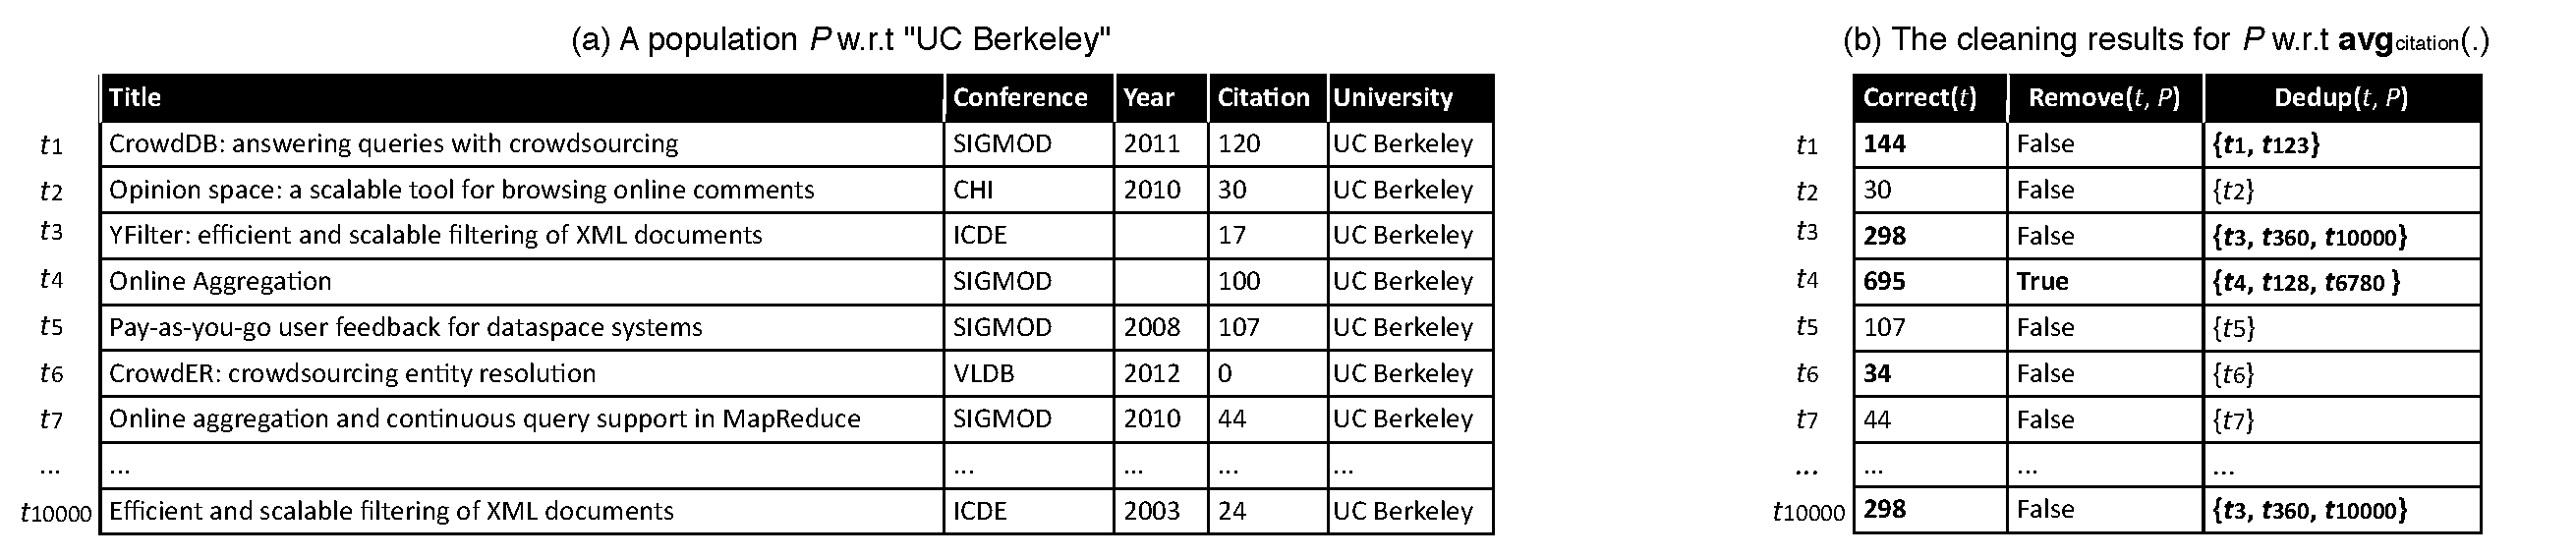
\includegraphics[scale=0.38]{figs/example.pdf}
\caption{A sample of dirty data and the corresponding clean data}
\label{fig:arch}
%\vspace*{-10pt}
\end{figure*}
\begin{example}

\end{example}
\fi
\iffalse
\projx supports a constrained set of SQL \groupby queries, which group tuples in a single table. In addition, \projx also allows users to add the time, cost and quality constraints to the queries. For example, consider the Publication. One example query over the table can be:  
\begin{alltt}
SELECT \textsf{AVG}(Citation) FROM Publication
WHERE year <= 2010
GROUP BY Conference
WITHIN COST 10000 TUPLES, TIME 30 MINUTES
\end{alltt}

    

\begin{alltt}
SELECT Aggregate(\(A\)) FROM Table
WHERE Predicate(\(B\sb{1},B\sb{2},...,B\sb{n}\))
GROUP BY \(C\sb{1},C\sb{2},...,C\sb{m}\)
WITHIN TIME t, ERROR e CONFIDENCE f (, COST c)
\end{alltt}



We start by introducing the BlinkDB extends SQL by enabling 
\begin{itemize}
  \item Group-by query with predicates
  \item Cost/Time/Quality Constraints
  \item \textsf{COUNT}, \textsf{AVG}, \textsf{SUM}, \textsf{STDDEV} and \textsf{VAR}
  \item For example:

  \item Maximize result quality:
  \begin{alltt}
SELECT \textsf{AVG}(Citation) FROM Publication
WHERE Conference = "\textsf{SIGMOD}"
WITHIN COST 1000 TUPLES, TIME 30 MINUTES
\end{alltt}
  \item Minimize cost and time:
  \begin{alltt}
SELECT \textsf{AVG}(Citation) FROM Publication
WHERE Conference = "\textsf{SIGMOD}"
WITHIN ERROR 0.1 CONFIDENCE 95%
\end{alltt}

\end{itemize}

\begin{alltt}
SELECT Aggregate(\(a\)) FROM \(T\)
WHERE Predicate(\(A\sb{p}\))
GROUP BY \(A\sb{g}\),
\end{alltt}

\fi
%Consider the following \groupby SQL query. The query allows users to specify cost, time, and quality constraints. Aggregate function can be \textsf{COUNT}, \textsf{AVG}, \textsf{SUM}, \textsf{STDDEV} and \textsf{VAR}. %To support \groupby queries, we can run the following query for each \groupby key.



%If the quality constraint is not specified, then the query aims to return the highest-quality answer within the cost and time constraints. For example,


%If the quality constraint is specified, then the query aims to spend the least cost and time to return the answer that satisfies the quality constraint. For example,





%WITHIN COST c, TIME t, ERROR e CONFIDENCE f;

%We assume If we are unable to return an answer that satisfies all constraints, we will find the result with the minimum error  Since it may be impossible to get a result that satisfies all constraints, we specify a priority for each constraint, and require that the query has to satisfy the constraints following their priorities. Here we suppose the order of the constraints represent their priorities.


